\setlength{\parskip}{\baselineskip} 
\section{Metodología}

\begin{frame}[c] 
\frametitle{}
\centering
\huge \textbf{Metodología para la resolución de problemas}
\end{frame}

\begin{frame}[t]
\frametitle{Metodología para la resolución de problemas}
\begin{block}{\textbf{Problema}}
Un problema se entiende como una proposición que, a partir de ciertas condiciones conocidas, induce a buscar algo desconocido.
\end{block}
El proceso de resolución de un problema con una computadora conduce a la escritura de un programa y a su ejecución en la misma. Aunque el proceso de diseñar programas es -esencialmente- un \textbf{proceso creativo}, se pueden considerar una serie de fases o pasos comunes a seguir.
\end{frame}

\begin{frame}[t]
\frametitle{Metodología para la resolución de problemas}
Las fases de resolución de un problema con computadora son:
\begin{itemize}
    \item Análisis del problema \pause
    \item Diseño del algoritmo \pause
    \item Codificación \pause
    \item Compilación y ejecución \pause
    \item Verificación \pause
    \item Depuración \pause
    \item Mantenimiento \pause
    \item Documentación
\end{itemize}
\end{frame}

\begin{frame}[t]
\frametitle{Análisis del problema}
\begin{itemize}
    \item Es la primera fase de la resolución de un problema con computadora.
    \item Requiere una clara definición de las \textbf{entradas} y \textbf{salidas}.
\end{itemize}
\textbf{Ejercicio:} Describa el proceso de retirar dinero del cajero.
\end{frame}

\begin{frame}[t]
\frametitle{Diseño del algoritmo}
\begin{block}{\textbf{Algoritmo}}
Un algoritmo es un \textcolor{orange}{conjunto de pasos}, procedimientos o acciones que nos permiten alcanzar un resultado o \textcolor{orange}{resolver un problema}.
\end{block}
Un algoritmo se puede concebir como un \textcolor{orange}{diálogo entre una computadora y una persona}, en el que se especifica bajo qué condiciones la computadora debe generar la salida específica.
\end{frame}

\begin{frame}[t]
\frametitle{Características de los algoritmos}
Las características que los algoritmos deben reunir son las siguientes:
\begin{itemize}
    \item \textcolor{blue}{Precisión:} los pasos a seguir en el algoritmo deben ser precisados claramente. \pause
    \item \textcolor{blue}{Determinismo:} dado un conjunto de datos idénticos de entrada, siempre debe arrojar los mismos resultados. \pause
    \item \textcolor{blue}{Finitud:} independientemente de su complejidad, siempre debe ser de longitud finita. 
\end{itemize}
\end{frame}

\begin{frame}[t]
\frametitle{Diagrama de flujo}
Un \textcolor{blue}{diagrama de flujo} representa la \textcolor{orange}{esquematización gráfica} de un algoritmo. Es decir, muestra gráficamente los pasos o procesos a seguir para alcanzar la \textcolor{orange}{solución de un problema}.
\end{frame}

\begin{frame}[t]
\frametitle{Símbolos utilizados en los diagramas de flujo}
\begin{center}
    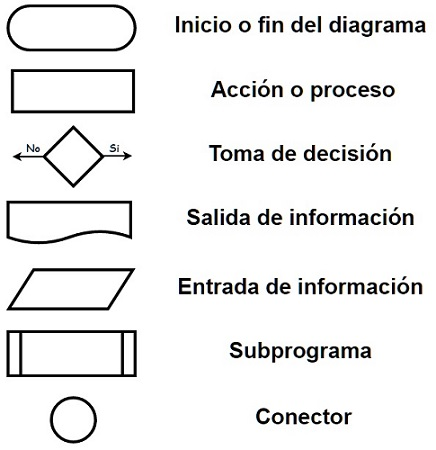
\includegraphics[width=0.57\textwidth]{figs/diagrama_flujo_simbolos}
\end{center}
\end{frame}

\begin{frame}[t]
\frametitle{Codificación}
\textcolor{blue}{Codificación} es la escritura en un lenguaje de programación de la representación del algoritmo desarrollada en etapas anteriores.
\end{frame}

\begin{frame}[t]
\frametitle{Depuración}
La \textcolor{blue}{depuración} es el proceso de encontrar los errores del programa y corregir o eliminar dichos errores.\\
Cuando se ejecuta un programa se pueden producir tres tipos de errores:
\begin{itemize}
    \item \textcolor{blue}{Errores de compilación:} o \textit{errores de sintaxis}, se producen normalmente por un uso incorrecto de las reglas del lenguaje de programación. \pause
    \item \textcolor{blue}{Errores de ejecución:} se producen por instrucciones que la computadora puede comprender pero no ejecutar (división por cero, raíces cuadradas de números negativos). \pause
    \item \textcolor{blue}{Errores lógicos:} se producen en la lógica del programa y la fuente del error suele ser el diseño del algoritmo.
\end{itemize}
\end{frame}


\begin{frame}[t]
\frametitle{Ejercicios}
Realiza el análisis, el algoritmo y el diagrama de flujo de los siguiente problemas:
\begin{itemize}
    \item Calcular la suma de dos números.
    \item Calcular el área de un triángulo.
    \item Calcular la hipotenusa de un triángulo.
    \item Identificar el mayor de dos números.
    \item Identificar el mayor de tres números.
    \item Imprimir los primeros diez números pares.
\end{itemize}
\end{frame}



%\begin{frame}
%\frametitle{Before Tao}
%	\begin{itemize}
% 	\item Facebook was storing the social graph to MySql
%	\begin{itemize}
%		\item  	Quering it from PHP
%		\item  	Storing result in memcache\\
%	\end{itemize}
%	\end{itemize}
%	\begin{center}
%		\includegraphics[width=0.3\textwidth]{figs/php-logo.eps}\quad
%		\includegraphics[width=0.3\textwidth]{figs/mysql.png}
%	\end{center}
% 	Over time Fb deprecated direct access to MySQL in favor of a graph (associations, nodes) abstraction
%\end{frame}



